\documentclass[10pt, margin=1mm,convert={density=500,outext=.png}]{standalone}
\usepackage{cmbright}
\usepackage[OT1]{fontenc}
\usepackage{graphicx}
\usepackage{amsmath}
\usepackage{booktabs}
\usepackage[table]{xcolor}
\usepackage{colortbl}


\graphicspath{ {../} }

% Try out cell padding to handle fractions
% Must prefix column formatters with `S'
\usepackage{cellspace}
\setlength\cellspacetoplimit{4pt}
\setlength\cellspacebottomlimit{4pt}

\definecolor{Gray}{gray}{0.95}
\newcolumntype{a}{>{\columncolor{Gray}}c}

\renewcommand{\familydefault}{\sfdefault}

% \setlength{\tabcolsep}{12pt}

\begin{document}
\small
\begin{tabular}{ccccc}
\toprule

% &
& \multicolumn{2}{c}{Offline Phase} & Online Phase\\
% \cmidrule(lr){3-4}\cmidrule(lr){5-5}
\cmidrule(lr){2-3}\cmidrule(lr){4-4}

% &
High-fidelity system & Snapshots & Projection & Emulation \\

% Steps
% &

$
\!\!
\begin{bmatrix}
\vcenter{\hbox{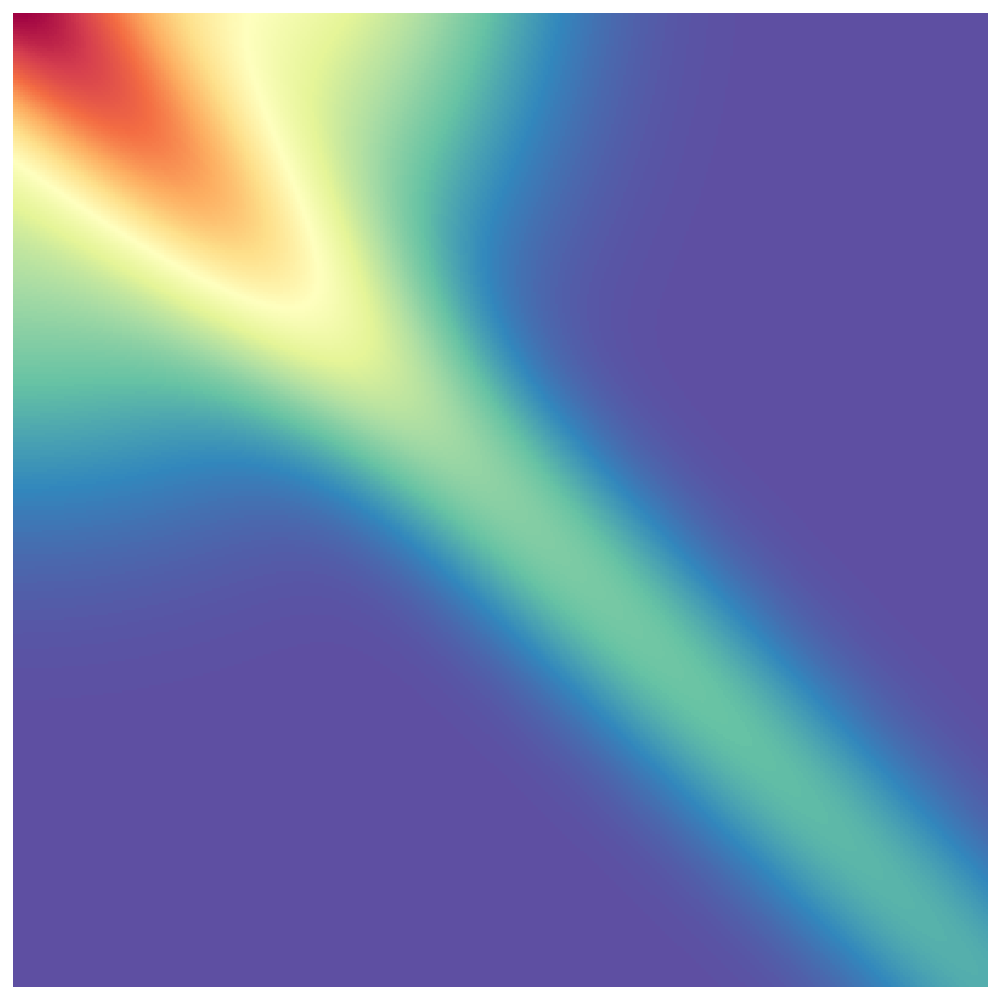
\includegraphics{highfidelity.png}}}
\end{bmatrix}
\!\!
\begin{bmatrix}
\vcenter{\hbox{
\includegraphics{wave_function.png}}}
\end{bmatrix}
\!\!
=
E
\begin{bmatrix}
\vcenter{\hbox{
\includegraphics{wave_function.png}}}
\end{bmatrix}
\!\!
$

&
$
% X =
\begin{bmatrix}
\vcenter{\hbox{
\includegraphics{basis.png}}}
\end{bmatrix}
$

&

$
\!\!
\begin{bmatrix}
\vcenter{\hbox{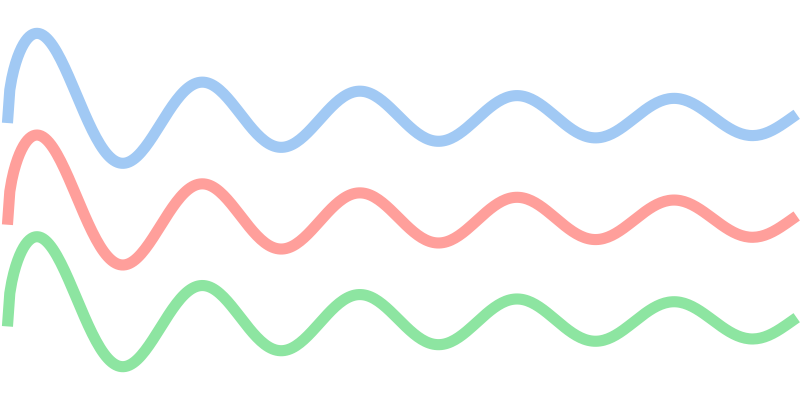
\includegraphics{basis_t.png}}}
\end{bmatrix}
\!\!
\begin{bmatrix}
\vcenter{\hbox{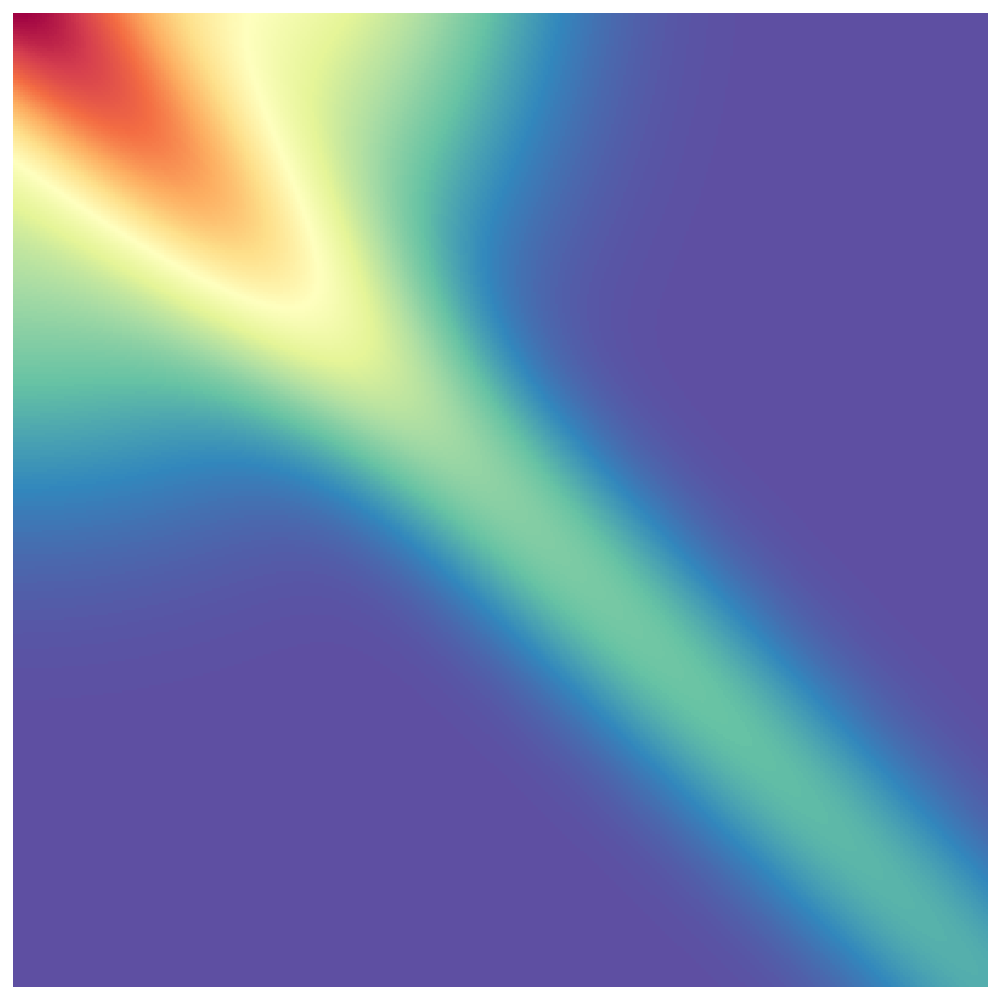
\includegraphics{highfidelity.png}}}
\end{bmatrix}
\!\!
\begin{bmatrix}
\vcenter{\hbox{
\includegraphics{basis.png}}}
\end{bmatrix}
\!\!
% \longrightarrow
=
\!\!
\begin{bmatrix}
\vcenter{\hbox{
\includegraphics{projected_matrix.png}}}
\end{bmatrix}
\!\!
$

&

$
\!\!
\begin{bmatrix}
\vcenter{\hbox{
\includegraphics{projected_matrix.png}}}
\end{bmatrix}
\!\!
\begin{bmatrix}
\vcenter{\hbox{
\includegraphics{coefficients.png}}}
\end{bmatrix}
\!\!
=
\widetilde E
\begin{bmatrix}
\vcenter{\hbox{
\includegraphics{coefficients.png}}}
\end{bmatrix}
\!\!
$
\\\midrule

% Time
% $t$
% &
Time:~
$\vcenter{\hbox{
\includegraphics{time_long.png}}}$ per evaluation &

$N_b \times \vcenter{\hbox{
\includegraphics{time_long.png}}}$

&

$\sim \vcenter{\hbox{
\includegraphics{time_long.png}}}$

&

Sampling: $\vcenter{\hbox{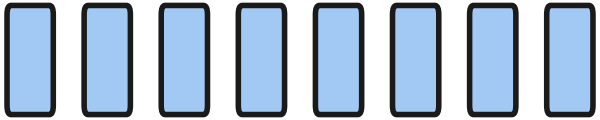
\includegraphics{time_short.png}}}$

\\

\bottomrule
\end{tabular}

\end{document}
